\documentclass[12pt]{article}

\usepackage[top=1in, bottom=1in, left=1in, right=1in]{geometry} 
\usepackage{graphicx}
\usepackage{setspace}
\usepackage{bm}
\usepackage{amsmath}
\usepackage{amssymb,amsmath}
\usepackage{listings}
\usepackage{color}
\usepackage{enumitem}
\usepackage{fancyvrb}
\usepackage{hyperref}
\usepackage{diagbox}
\geometry{letterpaper}
\linespread{1.1}% \geometry{landscape} % rotated page geometry

\definecolor{codegreen}{rgb}{0,0.6,0}
\definecolor{codegray}{rgb}{0.5,0.5,0.5}
\definecolor{codepurple}{rgb}{0.58,0,0.82}
\definecolor{backcolour}{rgb}{0.95,0.95,0.92}
\definecolor{outcolor}{rgb}{0.545, 0.0, 0.0}

\lstdefinestyle{mystyle}{
	backgroundcolor=\color{backcolour},   
	commentstyle=\color{codegreen},
	keywordstyle=\color{magenta},
	numberstyle=\tiny\color{codegray},
	stringstyle=\color{codepurple},
	basicstyle=\footnotesize,
	breakatwhitespace=false,         
	breaklines=true,                 
	captionpos=b,                    
	keepspaces=true,                 
	numbers=left,                    
	numbersep=5pt,                  
	showspaces=false,                
	showstringspaces=false,
	showtabs=false,                  
	tabsize=2
}

\lstset{style=mystyle}

\title{HW 1: Battery Modeling, Analysis, and Simulation}
\date{2 Feb. 2018} 
\author{Franklin Zhao \\ SID: 3033030808}

\begin{document}
	
	\maketitle
	\newcommand{\tabitem}{~~\llap{\textbullet}~~}
	\renewcommand\theequation{\arabic{equation}}
	\renewcommand{\figurename}{Fig.}
	\renewcommand\thesection{Problem \arabic{section}:}
	\renewcommand\thesubsection{(\alph{subsection})}
	\onehalfspacing
	
\section{Review Submission Procedure from HW0}
\section{Reading}
The first issue is decarbonization, which is the main driver for the smart grid development. With the growing concerns over energy scurity and global climate change, interest in renewables is increasing significantly. More significant progress will be made in understanding of environmental issues and using electricity innovations to reslove the energy issue. The second issue is reliability in the face of growing demand. With the increasing stress in electric grid, a question whether carrying capacity or safety margin will exist to satisify the demand is raised. The third issue is the electrification of transportation. Next-generation transportation systems will depend more electricity supplied by the grid. The fourth issue is that consumers have more power. The size of system peak influences the capacity needs to be built, and short timescale variability determines the flexibility required to follow the demand. The last issues are market designs and regulatory paradigms. New market designs have pushed the system upgrade and investment by allowing competition in several economy strategic sectors.\footnote{Annaswamy, A. M. ``Vision for smart grid control: 2030 and beyond." \textit{IEEE Standards Publication} (2013).}\\\\
In terms of the growing demand of consumers, for example, we can minimize a cost function from the view of the utility operator or the consumer, and review fundamental problems in energy storage management. To achieve the optimization objective,
we can focus on deciding when and how much to charge and discharge the battery, either in terms of a mismatch between energy supply and demand or the cost.\footnote{Koutsopoulos, Iordanis, Thanasis G. Papaioannou, and Vasiliki Hatzi. ``Modeling and optimization of the smart grid ecosystem." \textit{Foundations and Trends$^{\tiny{\textregistered}}$ in Networking} 10.2-3 (2016): 115-316.}
\section{Black-box vs. White-box Modeling}
The answer\footnote{http://www.idc-online.com/technical\_references/pdfs/electronic\_engineering/Modelling\_Choosing\_a\_Model.pdf} is shown in Table~\ref{tb:p3}.
\begin{table}[!htb]
\centering
\caption{\label{tb:p3}Black-box vs. White-box}
\vspace{5pt}
\begin{tabular}{|c|l|l|}
\hline
\hline
\diagbox[width=7.2em] & \multicolumn{1}{c|}{\textbf{Black-Box Models}} & \multicolumn{1}{c|}{\textbf{White-Box Models}}\\
\hline
& \tabitem Useful for training data rigime &\tabitem Insight into internal phenomena\\
Advantages & \tabitem No domain knowledge needed &\tabitem Extrapolation can be done\\
& \tabitem Minimal required computing power & \tabitem Very close to actual behavior\\
\hline
& \tabitem Lack of flexibility &\tabitem May be very complex\\
Disadvantages & \tabitem Lack of physical meaning & \tabitem Restricted to assumed structure\\
& \tabitem Not good for sensitivity analysis &\tabitem 
Large computing overheads\\
\hline
\hline
\end{tabular}
\end{table}
\section{Mathematical Modeling Use}
The five potential uses are listed as follows\footnote{Moura, S. J. ``Ch1: Modeling Systems" \textit{CE 295 Lecture Notes} (2018).}:
\begin{itemize}[noitemsep, topsep=0pt]
	\item[{\textbf{1}}] \textbf{Analysis.} Given a future trajectory of $u(t)$, $x(0)$ at the present, and the system model $\Sigma$, predict the future of $y(t)$.
	\item[{\textbf{2}}] \textbf{State Estimation.} Given a system $\Sigma$ with time histories $u(t)$ and $y(t)$, find $x$ that is consistent with $\Sigma$, $u$, $y$.
	\item[{\textbf{3}}] \textbf{System Design or Planning.} Given $u(t)$ and some desired $y(t)$, find $\Sigma$ such that $u(t)$ acting on $\Sigma$ will produce $y(t)$.
	\item[{\textbf{4}}] \textbf{Model Identification.} Given time histories $u(t)$ and $y(t)$, usually obtained from experimental data, determine a model $\Sigma$ and its parameter values that are consistent with $u$ and $y$.
	\item[{\textbf{5}}] \textbf{Control Synthesis.} Given a system $\Sigma$ with current state $x(0)$ and some desired $y(t)$, find $u(t)$ such that $\Sigma$ will produce $y(t)$. 
\end{itemize}
\section{Methematical Modeling}
\subsection{}
``Reservoirs"(States): State-of-charge $\bf{z(t)}$ and capacitor voltage $\bf{V_c(t)}$.
\subsection{}
According to Kirchoff's voltage and current laws, the following systems equations and integrator dynamics can be derived:
\begin{eqnarray}
V(t)-OCV(z)-V_C(t)-R_1I(t)=0\\
I(t)=C\dot{V_C}(t)+\frac{V_C(t)}{R_2}\\
\dot{z}(t)=\frac{1}{Q}I(t)
\end{eqnarray}
\subsection{}
Parameters: Voltage source $\bf{OCV(z)}$, Resistance $\bf{R_1}$ and $\bf{R_2}$, Capacity $C$, and charge capacity $Q$.
\subsection{}
State space form:
\begin{eqnarray}
\dot{z}(t)=\frac{1}{Q}I(t)\\
\dot{V_C}(t)=-\frac{1}{R_2C}V_C(t)+\frac{1}{C}I(t)\\
V(t)=OCV(z)+V_C(t)+R_1I(t)\label{eq:out}
\end{eqnarray}
\subsection{}
Denote $[z(t),\ V_C(t)]^T$ by $X$; Denote $I$ by $u$. The state equations can be written as:
\begin{equation}
\dot{X}=AX+Bu
\end{equation}
It is a linear state equation, where
\begin{equation*}
A=\left[
\begin{array}{cc}
0 & 0\\
0 & -\frac{1}{R_2C} 
\end{array}\right]\ \text{and}\ B=\left[
\begin{array}{c}
\frac{1}{Q}\\
\frac{1}{C}
\end{array}\right]
\end{equation*}
However, the model does \textbf{not} have a linear output equation, since the $\bf{OCV(z)}$ term produces nonlinearity.
\section{Stability and Linearization}
\subsection{}
From the last problem we know that the matrix $A$ is:
\begin{equation*}
\left[\begin{array}{cc}
0 & 0\\
0 & -\frac{1}{R_2C} 
\end{array}\right]
\end{equation*}
where we could easily identify that the eigenvalues are $\lambda_1=0$ and $\lambda_2=-\frac{1}{R_2C}$. Since $\lambda_1=0$ and $\lambda_2<0$, we can conclude that the model is \textbf{marginally stable}.
\subsection{}
Now let's perturbate a little around equilibrium:
\begin{align}
V=V^{eq}+\tilde{V}\\
V_C=V_C^{eq}+\tilde{V_C}\\
I=I^{eq}+\tilde{I}\\
z=z^{eq}+\tilde{z}
\end{align}
From Equation~\ref{eq:out}, the output equation can be derived:
\begin{equation}
\begin{array}{ll}
V&\approx V^{eq}+\tilde{V_c}\frac{\partial V}{\partial V_C}\Big{|}_{V_C^{eq}}+(I-I^{eq})\frac{\partial V}{\partial I}\Big{|}_{I^{eq}}+(z-z^{eq})\frac{\partial V}{\partial z}\Big|_{z^{eq}}\\
&=V^{eq}+(V_C-V_C^{eq})\frac{\partial V}{\partial V_C}\Big{|}_{V_C^{eq}}+(I-I^{eq})\frac{\partial V}{\partial I}\Big{|}_{I^{eq}}+(z-z^{eq})\frac{\partial V}{\partial z}\Big|_{z^{eq}}\\
&=V_C^{eq}+R_1\times I^{eq}+(p_0+p_1z^{eq}+p_2{z^{eq}}^2+p_3{z^{eq}}^3)+(V_C-0)\times 1+(I-0)\times R_1+\\
&\ \ \ (z-0.5)(p_1+2p_2\times 0.5+3p_3\times 0.5^2)\\
&=V_C+0.05I+(z-0.5)(p_1+p_2+0.75p_3)+(p_0+0.5p_1+0.25p_2+0.125p_3)\\
&=V_C+(p_1+p_2+0.75p_3)z+0.05I+(p_0-0.25p_2-0.25p_3)
\end{array}
\end{equation}
which becomes a linear equation.
\section{Simulation and Analysis}
\subsection{}
\lstinputlisting[language=Python]{7a.py}
The plot of nonlinear OCV functions vs. state-of-charge is shown in Figure~\ref{fig:OCVnl}.
\begin{figure}[!htb]
	\centering
	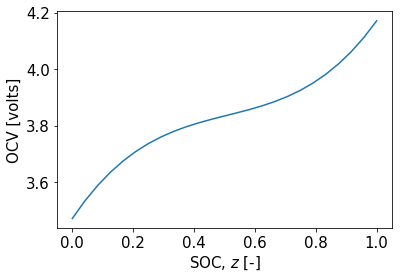
\includegraphics[width=10cm]{7a.png}      
	\caption{Nonlinear OCV functions vs. state-of-charge}
	\label{fig:OCVnl}
\end{figure}
\subsection{}
\lstinputlisting[language=Python]{7b.py}
The subplots are shown in Figure~\ref{fig:sim}.\\\\
\begin{figure}[!htb]
	\centering
	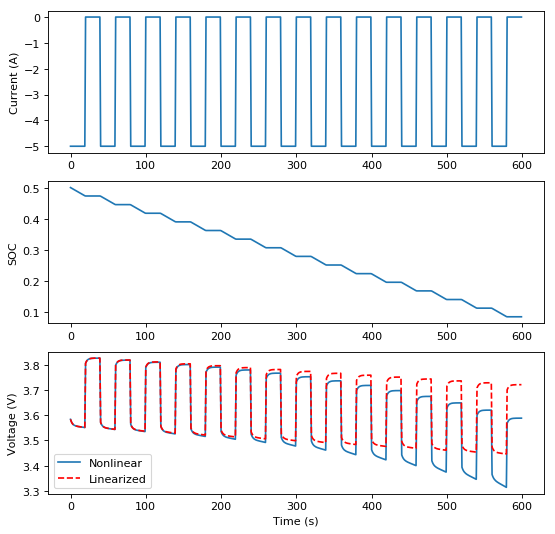
\includegraphics[width=15cm]{7b.png}      
	\caption{Current, SOC, and voltage vs. time}
	\label{fig:sim}
\end{figure}
\subsection{}
From the OCV and SOC plots in Figure~\ref{fig:OCVnl} and Figure~\ref{fig:sim}, we could see that when SOC drops below 25\%, the nonlinearity of OCV starts increasing dramatically (i.e., the inflection point is around 0.25), which means the system will continue moving away from the linearization point over time. Such results indicate that the linearized model performs well only within a small range, which means the perturbation cannot be too large. If we would like to study a wide range, new linearized models should be made in every small intervals. 
\end{document}